\section{Tree Decompositions Lab}
\label{sec:tree-decompositions-lab}

\textbf{Nozione}: I problemi NP-Hard sugli \textbf{alberi} sono più semplici da risolvere rispetto ai grafi.
Ma per quale motivo questa cosa funziona?

\subsection{Maximum Independent Set (MIS)}

Da scriver.

La soluzione per questo problema sfrutta la \textbf{programmazione dinamica}
come approccio. Si risolvono dei sotto-problemi per poi risolvere il problema
principale.

%albero con 1 nodo radice e 3 nodi figli
%per ogni nodo figlio ci sono 2 nodi figli

\begin{figure}[H]
    \begin{center}
        \begin{forest}
            for tree={circle,draw, l sep=20pt}
            [r
                [1
                        [1.1]
                        [1.2]
                ]
                [v
                        [2.1
                                [2.1.1]
                                [2.1.2]
                        ]
                        [2.2]
                ]
                [3
                        [3.1]
                        [3.2]
                ]
            ]
        \end{forest}
    \end{center}
\end{figure}

\[
    MIS(v) = MIS(T_{v,1}) + MIS(T_{v,2}) + MIS(T_{v,3}) \pm v
\]

\subsubsection{L'algoritmo di programmazione dinamica}

Per ogni vertice $v$ calcoliamo:
\begin{itemize}
    \item $M^+[v]$ = $|MIS(T_v) \cup \{v\}|$
    \item $M^-[v]$ = $|MIS(T_v) \setminus \{v\}|$
\end{itemize}

Per un vertice $v$ con figli $w_1, \dots, w_kd$:
\begin{itemize}
    \item $M^+[v] = 1 + \sum_{i=1}^d M^-[w_i]$
    \item $M^-[v] = \sum_{i=1}^d \max\{M^+[w_i], M^-[w_i]\}$
\end{itemize}

Quindi:
\[
    MIS(T) = \max{\{M^+[r], M^-[r]\}}
\]

Praticamente, quello che si fa è \textbf{calcolare il MIS per ogni
    sotto-albero} e poi si sommano i risultati per ottenere il \textbf{MIS
    dell'albero completo}.

L'algoritmo, praticamente, parte dalle \textbf{foglie} e risale verso la
\textbf{radice}.

\begin{esempio}(MIS su un albero facile)
\end{esempio}

%albero con 1 nodo radice e 2 nodi figli
%figlio sinistor ha 2 figli
%numerali in ordnie crescente

\begin{figure}[H]
    \begin{center}
        \begin{forest}
            for tree={circle,draw, l sep=20pt}
            [1
                [2
                        [4]
                        [5]
                ]
                [3]
            ]
        \end{forest}
    \end{center}
\end{figure}

Eseguendo l'algoritmo si ottiene:

\begin{itemize}
    \item \textbf{Nodo 4}:
          \begin{itemize}
              \item $M^+[4] = 1$
              \item $M^-[4] = 0$
          \end{itemize}
    \item \textbf{Nodo 5}:
          \begin{itemize}
              \item $M^+[5] = 1$
              \item $M^-[5] = 0$
          \end{itemize}

    \item \textbf{Nodo 2}:
          \begin{itemize}
              \item $M^+[2] = 1$
              \item $M^-[2] = 2$
          \end{itemize}

    \item \textbf{Nodo 3}:
          \begin{itemize}
              \item $M^+[3] = 1$
              \item $M^-[3] = 0$
          \end{itemize}

    \item \textbf{Nodo 1}:
          \begin{itemize}
              \item $M^+[1] = 1+2 = 3$
              \item $M^-[1] = 3$
          \end{itemize}
\end{itemize}

E cosa ci muoviamo in un caso del genere?

%inserisci immagine clique.png

\begin{figure}[H]
    \begin{center}
        \includegraphics[scale=0.5]{chapters/images/mis clique.png}
    \end{center}
\end{figure}

Se notiamo, possiamo dividere il problema in sotto-problemi.

\begin{figure}
    \begin{center}
        \includegraphics[scale=0.5]{chapters/images/clique format.png}
    \end{center}
    \caption{Formato del problema}
\end{figure}

\textbf{Intuizione}: Possiamo rappresentare un \textbf{grafo} $G$ come un albero $T$. I nodi di $T$ sono dei piccoli
moduli che chiamiamo \textbf{bags}. In questo caso, li trattiamo come \textit{sotto-problemi}.

Utilizziamo la programmazione dinamica per risolvere la tree decomposition.

Copiare grafico di Tree Decomposition: intuition

\begin{definition}(Tree Decomposition)
    Una tree decomposition di un grafo $G = (V,E)$ è un albero $T$ di bags $X$:
    \begin{itemize}
        \item se $(u,v) \in E$ allora $u$ e $v$ sono nella stessa bag.
        \item $\forall v \in V$ i bags che contengono $v$ sono connessi in $T$
    \end{itemize}

    Un grafo può ammettere diverse tree decomposition.
\end{definition}

\begin{definition}(Tree width)
    La treewidth è la width minore possibile tra tutti le tree decomposition ammesse nel grafo.

    Un po' di notazione:
    \begin{itemize}
        \item $tw(G)$ = treewidth di $G$
        \item $tw(G) = 1 \iff  G$ è una \textbf{foresta}
        \item $tw(G) = 2 \iff G$ è una serie di grafi paralleli
        \item Eliminare un arco in $G$ non aumneta la treewidth
        \item Contrarre archi non aumenta la treewidth
        \item Ogni cricca in $G$ deve essere contenuta in una bag
    \end{itemize}
\end{definition}

\subsection{Cops e Robber}
Abbiamo questo problema che viene definito in questo modo.

\begin{itemize}
    \item \textbf{1 Ladro} che si muove sul grafo.
    \item $k$ poliziotti che si muovono sul grafo.
    \item Per vincere, i poliziotti devono catturare il ladro e arrivare al suo nodo.
\end{itemize}

\begin{theorem}(Cops e Robber Condition)
    $tw(g) \leq k \iff k+1$ poliziotti possono vincere il gioco.

    La strategia è data dalla \textbf{tree decomposition}
\end{theorem}

Ci sono delle foto sulle slide. Poi vedo come fare.

\subsection{Calcolare la tree decomposition}

Si usano 2 concetti principali: \textbf{rimuovere un nodo} e
\textbf{triangolazione dei vicini} per costruire le bags.

\begin{definition}(Triangolazione dei vicini e rimozione dei nodi)
    Un grafo $G$ è \textbf{triangolato} se il ciclo più piccolo all'interno del $grafo$ ha lunghezza 3. (Da controllare)
    \begin{figure}[H]
        \begin{center}
            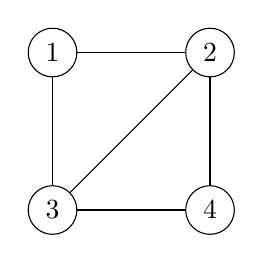
\begin{tikzpicture}
                \node[shape=circle,draw=black] (1) at (0,0) {1};
                \node[shape=circle,draw=black] (2) at (2,0) {2};
                \node[shape=circle,draw=black] (3) at (0,-2) {3};
                \node[shape=circle,draw=black] (4) at (2,-2) {4};

                \path [-] (1) edge node[left] {} (2);
                \path [-] (1) edge node[left] {} (3);
                \path [-] (2) edge node[left] {} (3);
                \path [-] (2) edge node[left] {} (4);
                \path [-] (3) edge node[left] {} (4);
            \end{tikzpicture}
        \end{center}
        \caption{Triangolazione}
    \end{figure}

    Per poter rimuovere un nodo $v$, se nel grafo $G$ rimuoviamo questo $v$, tutti
    i vicini di v $neig(v)$ devono essere tutti connessi tra loro.

    Ad esempio, nel grafo sopra, possiamo rimuovere in un caso il nodo $1$ e nel
    secondo caso il nodo $4$.

    \begin{figure}[H]
        \begin{center}
            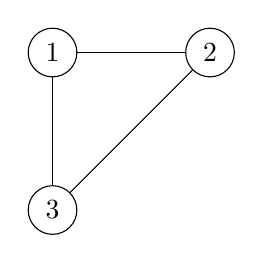
\begin{tikzpicture}
                \node[shape=circle,draw=black] (1) at (0,0) {1};
                \node[shape=circle,draw=black] (2) at (2,0) {2};
                \node[shape=circle,draw=black] (3) at (0,-2) {3};

                \path [-] (1) edge node[left] {} (2);
                \path [-] (1) edge node[left] {} (3);
                \path [-] (2) edge node[left] {} (3);
            \end{tikzpicture}
        \end{center}
        \caption{Triangolazione senza Nodo 4}
    \end{figure}

    \begin{figure}[H]
        \begin{center}
            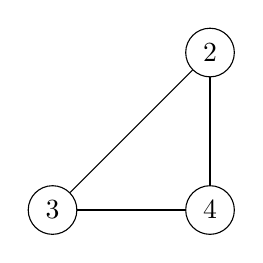
\begin{tikzpicture}
                \node[shape=circle,draw=black] (2) at (2,0) {2};
                \node[shape=circle,draw=black] (3) at (0,-2) {3};
                \node[shape=circle,draw=black] (4) at (2,-2) {4};

                \path [-] (2) edge node[left] {} (3);
                \path [-] (2) edge node[left] {} (4);
                \path [-] (3) edge node[left] {} (4);
            \end{tikzpicture}
        \end{center}
        \caption{Triangolazione senza Nodo 1}
    \end{figure}

    \begin{figure}[H]
        \begin{center}
            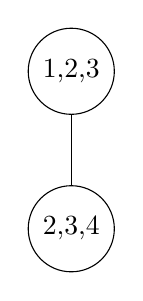
\begin{tikzpicture}
                \node[shape=circle,draw=black] (2) at (0,0) {1,2,3};
                \node[shape=circle,draw=black] (3) at (0,-2) {2,3,4};

                \path [-] (2) edge node[left] {} (3);
            \end{tikzpicture}
        \end{center}
        \caption{Perfect Elimination Order}
    \end{figure}

    I nodi che possono essere rimossi si chiamano \textbf{simplicial node}.

    Quindi, la migliore tree decomposition con la migliore treewidth si riduce a
    trovare la \textbf{PEO} (Perfect Elimination Order)
\end{definition}

Torniamo ora al \textbf{calcolo} della tree decomposition. Partiamo da un
\textbf{removal order} per un grafo.

Disegnare il grafo o mettere qualcos
\[
    removal\_order = [6,7,9,1,8,2,0,3,5,4]
\]

Praticamente, $\forall v \in removal\_order$: rimuovi $v$ e triangola i vicini.
Se i vicini sono già triangolati, si $crea$ la $bag$.

Vedere come fare per disegnare la tree decomposition. perché sono tantissimi
passaggi.

\textbf{Nota:} Quando si arriva a $\{3,4,5\}$ notiamo che esise già una bag più grande che è $\{0,3,4,5\}$ e non ci serve
quindi crearne un'altra.

\textbf{Risultato:} Abbiamo ottenuto una tree decomposition!

La domanda ora è: \textbf{Come otteniamo il \textit{removal order}}?

Il \textbf{calcolo} del removal order è un problema \textbf{NP-Hard}. Ci sono
$N!$ possibili ordini e $\mathcal{O}(2^n)$ con la programmazione dinamica.

Per risolvere questo problema, quindi, è usare un'euristica per trovare delle
\textbf{soluzioni accettabili}.

\begin{definition}(Minimum degree heuristic)
    Quando rimuoviamo un nodo dalla tree decomposition, rimuoviamo il nodo che ha il \textbf{grado minore}, cioé il nodo
    che ha il \textbf{minor numero di vicini}.

    Rimuovere un nodo cambia anche il \textbf{grado} dei vicini e quindi calcoliamo
    il \textbf{minimum degree} ad ogni iterazione.
\end{definition}

Di fatto, il removal order di prima è stato calcolato sfruttando questa
\textbf{minimum degree heuristic}. \newpage